\documentclass{uofa-eng-assignment}

\usepackage{lipsum}
\usepackage{wrapfig}
\usepackage{caption}
\usepackage{subcaption}
\usepackage{float}
\usepackage[portuguese]{babel}
\usepackage[numbib]{tocbibind}
\usepackage{hyperref}

\newcommand*{\course}{Metodologias Experimentais em Informática}
\newcommand*{\assignment}{Assignment 1 v2 - Análise Exploratória de Dados}

\begin{document}

%\begin{flushright}\hspace{-1.5cm}\vspace{-1.6cm}
%    
\includegraphics[height=1.5cm]{fctuc.png}
%\end{flushright}

\begin{center}
    \textbf{\large \course}\\
    \assignment
\end{center}

\begin{center}
\begin{minipage}{0.3\textwidth}
\begin{center}Francisco Pires\\2019201225\\fjrp@student.dei.uc.pt\end{center}
\end{minipage}
\begin{minipage}{0.3\textwidth}
\begin{center}Gonçalo Pereira\\2008119715\\gnsp@student.dei.uc.pt\end{center}
\end{minipage}
\begin{minipage}{0.3\textwidth}
\begin{center}Tiago Delgado\\2021179681\\tiagodelgado@student.dei.uc.pt\end{center}
\end{minipage}
\end{center}

{\centering Repositório do projeto: \emph{github.com/goncalonsp/mei-2022-2023}\par }

\rule{0.9\linewidth}{0.1mm}

\section{Introdução }

Este trabalho foi realizado no âmbito da cadeira de Metodologias Experimentais em Informática e tem como objetivo estudo do Problema do Fluxo Máximo, ou Maximum Flow Problem, em Inglês. Este problema tem como objectivo a descoberta e maximização de uma taxa de fluxo numa determinada rede de fluxo. Um exemplo da aplicabilidade e importância do estudo deste problema é o seu uso no escalonamento da indústria aeronáutica. Nesse caso é considerado o grafo do conjunto de voos entre nós, os aeroportos, sendo que cada voo parte e tem destino num nó. Como variável de fluxo temos as equipas de tripulação necessárias para operar os voos.
No âmbito deste trabalho consideramos uma aplicação mais simples e abstrata onde temos as seguintes variáveis:
\begin{itemize}
\item $n$ = número de vértices
\item $p$ = probabilidade de criação de arco entre vértices, $0 \leq p \leq 1$
\item $r$ = capacidade de fluxo máxima
\item $s$ = seed aleatória, usada para geração aleatória dos grafos para experiência
\item $|A|$ = número de arcos, estimado como $|A|=p\frac{n(n-1)}{2}$.
\end{itemize}
Neste estudo vamos considerar 3 implementações para o Problema do Fluxo Máximo: o algoritmo Dinic; o algoritmo Edmond-Karp (doravante referido como ``EK''); e o algoritmo Malhotra, Pramodh-Kumar and Maheshwari (referido como ``MPM'').
Todos os tempos de execução são apresentados em segundos.
Também foi disponibilizado um input data generator aleatório para os respetivos inputs em python (\texttt{gen.py}), onde foi necessário definir as variáveis $n$, $p$, $r$, $s$, e o nome do ficheiro que contém os dados de entrada.

\section{Cenários de Teste }

Para realizar os testes, criámos um programa (\texttt{executor.py}) que recebe como parâmetro o nome do ficheiro CSV de entrada, que possui todos os dados para a geração (n, p, r, s), e também o nome que queremos dar ao ficheiro CSV de saída. Este ficheiro de saída vai possuir todos os dados do ficheiro de entrada e ainda 3 colunas adicionais que correspondem aos valores de tempo dos 3 algoritmos. 
Para definir os valores a usar das várias variáveis, realizamos uma série de testes exploratórios iniciais para perceber o comportamento de cada algoritmo. Depressa chegamos à conclusão que os algoritmos apresentam desempenhos diferentes e portanto optamos por utilizar intervalos diferentes para cada algoritmo. Optámos ainda por ignorar intervalos que produzissem tempos de execução inferiores a 10 milissegundos, sob pretexto que o objetivo é medir a performance do algoritmo e não variações associadas à execução computacional (latências de input/output, concorrência de recursos, etc…).
No final dos testes exploratórios iniciais, ficámos com os seguintes intervalos:
\begin{itemize}
\item Dinic: $n\in[1000,10000]$; EK: $n\in[400,1500]$; MPM: $n\in[1000,5000]$. 
\item Dinic, MPM e EK: $p=\{0.1, 0.2, 0.3, ..., 0.9\}$.
\item $r=n$
\item $s$ foi sempre aleatório.
\end{itemize}

\section{Procedimentos e Resultados dos Testes }
\subsection{Variáveis Dependentes e Independentes }

Para objeto de estudo, foram selecionadas três variáveis principais, sendo que a variável dependente corresponde ao tempo em segundos que o algoritmo demora a executar, isto é, a executar e extrair os dados para objeto de estudo. Para as variáveis independentes considerámos $n$ e $p$.
Pretende-se com esta análise exploratória dos dados, obter uma melhor visão do problema, com a finalidade de obter conclusões relativas aos três algoritmos e avaliar a sua performance perante o cenário de teste considerado.

\subsection{Amostragem dos resultados e interpretação }

Após a realização de testes para os três algoritmos, obtemos o nosso dataset que corresponde aos dados obtidos pelos testes, destacamos  3 variáveis utilizadas para objeto de estudo: o número de vértices, a probabilidade e o $A$ (número de arestas). A nossa variável dependente (tempo de execução) varia entre 0.00001 e 1000 segundos (sendo que 1000 significa que não foi encontrada uma solução perante o cut-off time).
A média de valores do tempo de execução para o algoritmo Dinic.cpp é a mais baixa entre os algoritmos testados e o algoritmo EK apresenta a média de valores mais altos.
Em relação ao algoritmo MPM a média de valores do tempo de execuções foi aproximadamente 3s mais alto em relação ao algoritmo Dinic.

\section{Visualização e Interpretação dos dados (EDA) }

A fim de retirar dos dados uma conclusão mais objetiva, decidimos realizar uma análise exploratória dos dados, denominada “EDA” (Exploratory Data Analysis), que consiste num conjunto de estatísticas e gráficos que revelam características sobre os dados. O objetivo da EDA passa por analisar, descobrir e identificar padrões, características, tendências e outliers, com a finalidade de obter o máximo de informações sobre a estrutura dos dados.
A informação relativa ao conjunto de dados é representada através de diferentes tipos de gráficos que permitem assim uma visualização  mais objetiva sobre as variáveis de estudo, relação entre as mesmas que posteriormente permitem a formulação de hipóteses e conclusões sobre o nosso estudo.

Analisando os boxplots das figuras \ref{fig:boxplot-dinic-n}, \ref{fig:boxplot-ek-n} e \ref{fig:boxplot-mpm-n}, observamos que, para todos os casos, a mediana, ou segundo quartil, aumenta progressivamente para valores maiores de $n$. Isto leva-nos a concluir que o nº de vértices, $n$, tem um impacto direto no tempo de execução. A mesma conclusão já não pode ser retirada das figuras \ref{fig:boxplot-dinic-p}, \ref{fig:boxplot-ek-p} e \ref{fig:boxplot-mpm-p}, onde se observa para o caso do algoritmo Dinic a mediana mantém-se inalterada com a variação de $p$. É importante ainda realçar que para o algoritmo MPM, embora a mediana pareça aumentar, o impacto de $p$ não é tão expressivo como para o algoritmo EK.

Continuando a analise dos bloxplots em função de $p$, podemos ainda observar um fenómeno particular para o algoritmo Dinic. Neste caso, e contrariamente a todos os outros, o aumento de $p$ parece gerar uma redução na variância do tempo de execução.

Finalmente, olhando apenas para os tempos de execução concluímos rapidamente que o algoritmo Dinic aparenta ser o mais performante dos três, conseguindo tempos manifestamente inferiores a 50 segundos para grafos com 10000 vértices.

\begin{figure}[h]
    \begin{minipage}{0.45\textwidth}
        \centering
        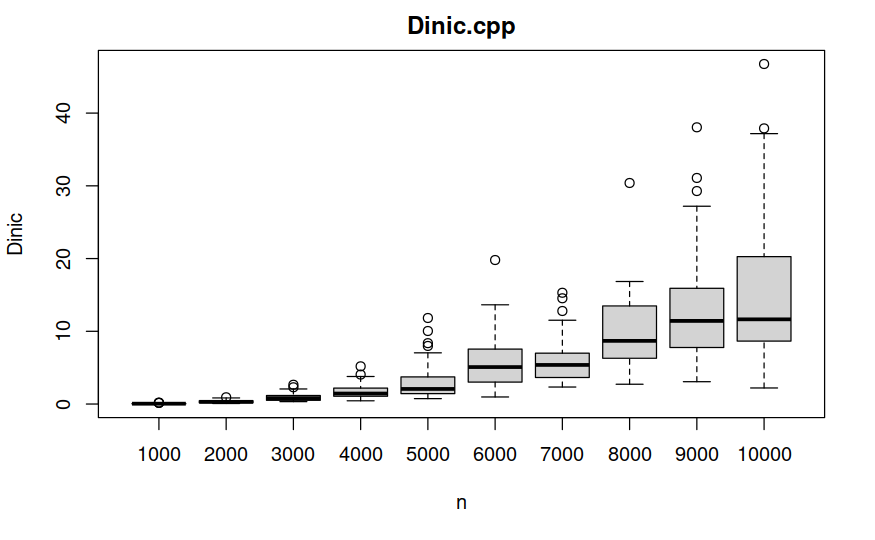
\includegraphics[width=1\textwidth]{boxplot_dinic_n.png}
        \caption{Dinic boxplot para $n$}
        \label{fig:boxplot-dinic-n}
    \end{minipage}
    \hfill
    \begin{minipage}{0.45\textwidth}
        \centering
        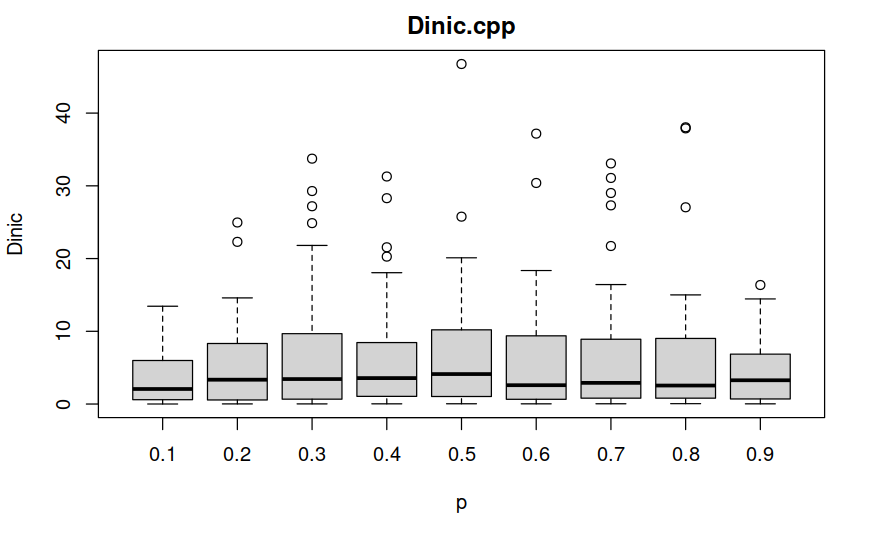
\includegraphics[width=1\textwidth]{boxplot_dinic_p.png}
        \caption{Dinic boxplot para $p$}
        \label{fig:boxplot-dinic-p}
    \end{minipage}
\end{figure}

\begin{figure}[h]
    \begin{minipage}{0.45\textwidth}
        \centering
        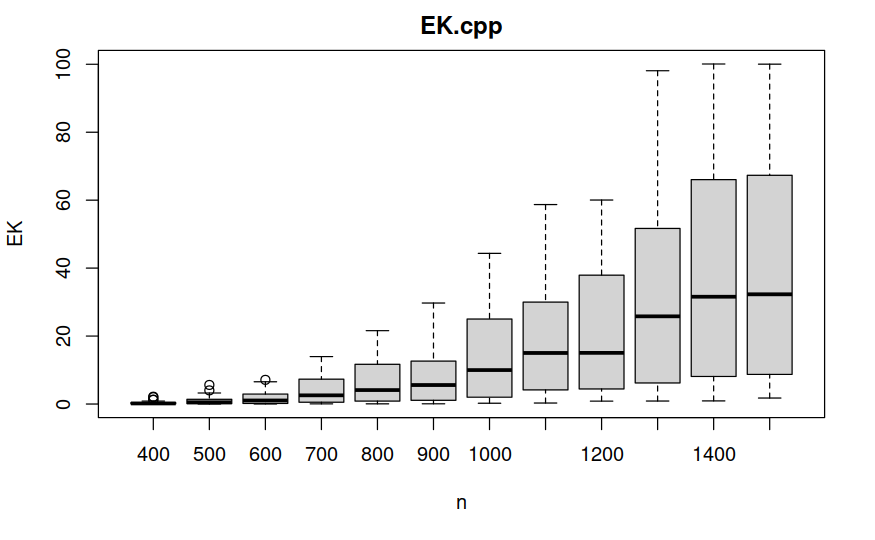
\includegraphics[width=1\textwidth]{boxplot_ek_n.png}
        \caption{EK boxplot para $n$}
        \label{fig:boxplot-ek-n}
    \end{minipage}
    \hfill
    \begin{minipage}{0.45\textwidth}
        \centering
        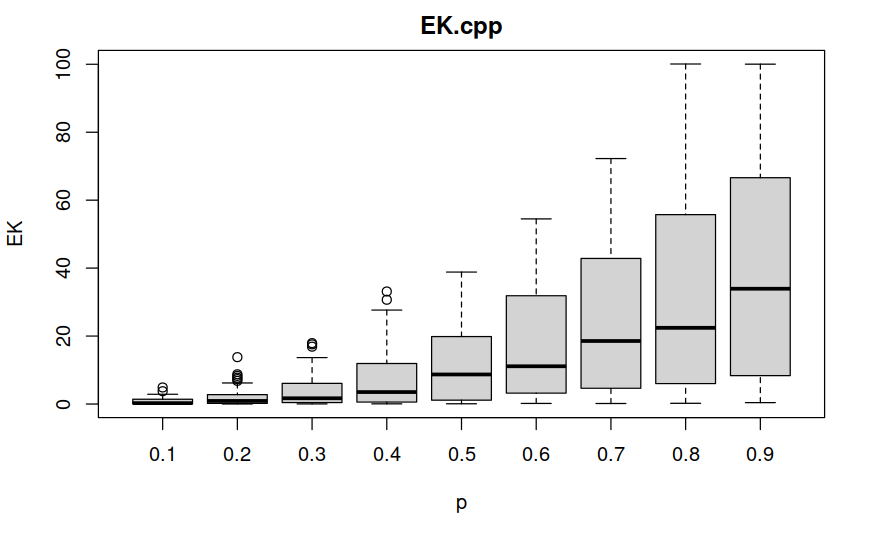
\includegraphics[width=1\textwidth]{boxplot_ek_p.png}
        \caption{EK boxplot para $p$}
        \label{fig:boxplot-ek-p}
    \end{minipage}
\end{figure}

\begin{figure}[h]
    \begin{minipage}{0.45\textwidth}
        \centering
        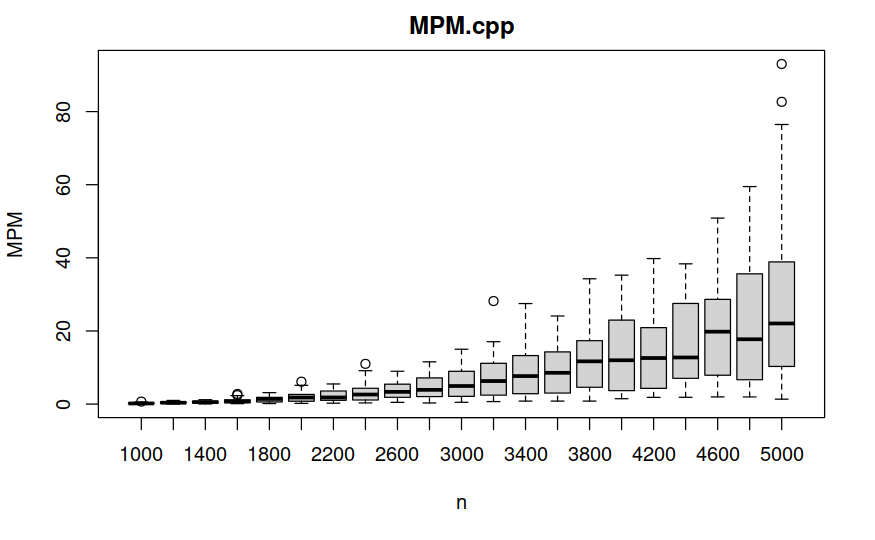
\includegraphics[width=1\textwidth]{boxplot_mpm_n.png}
        \caption{MPM boxplot para $n$}
        \label{fig:boxplot-mpm-n}
    \end{minipage}
    \hfill
    \begin{minipage}{0.45\textwidth}
        \centering
        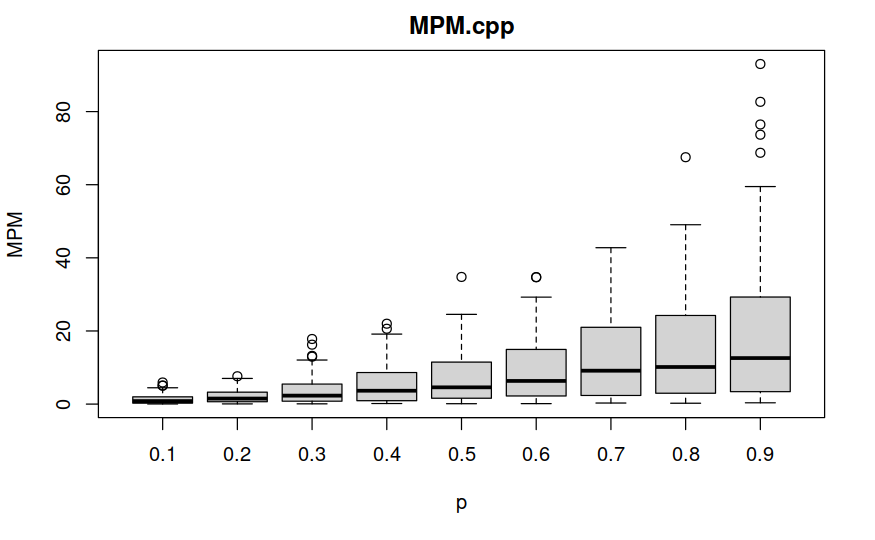
\includegraphics[width=1\textwidth]{boxplot_mpm_p.png}
        \caption{MPM boxplot para $p$}
        \label{fig:boxplot-mpm-p}
    \end{minipage}
\end{figure}






\newpage\clearpage
\section{Regressão Linear}

Em seguida é mostrado o modelo de regressão linear. Sabemos que o algoritmo Dinic e EK tem uma complexidade temporal de $O(|A||V|^2)$ e $O(|V||A|^2)$, por isso começamos por encaixá-los em funções quadráticas da mesma forma (ver figura \ref{fig:dinic-regression} e \ref{fig:ek-regression}). Relembramos o leitor que $A$ foi estimado como $|A|=p\frac{n(n-1)}{2}$.
\begin{figure}[h]
    \centering
    \begin{minipage}{0.45\textwidth}
        \centering
        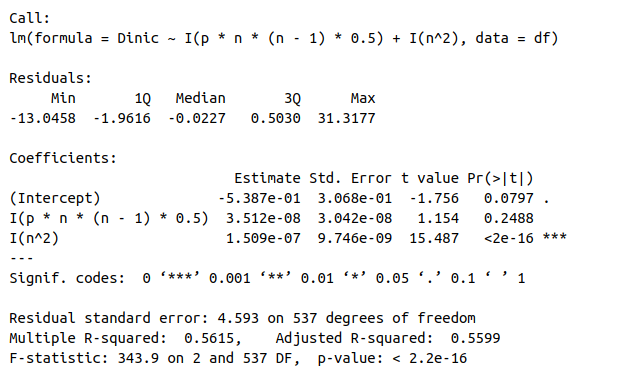
\includegraphics[width=1.1\textwidth]{dinic_a+n^2_lm.png}
        \captionsetup{justification=centering}
        \caption{Resultado da regressão linear: \\$Dinic \sim a + n^2$}
        \label{fig:dinic-regression}
    \end{minipage}
    \hfill
    \begin{minipage}{0.45\textwidth}
        \centering
        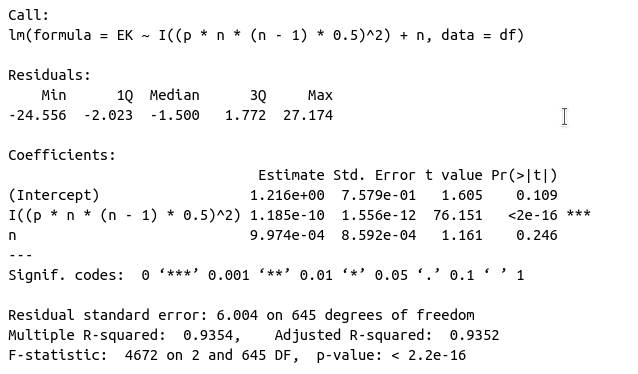
\includegraphics[width=1.1\textwidth]{ek_a^2+n_lm.png}
        \captionsetup{justification=centering}
        \caption{Resultado da regressão linear: \\$EK \sim a^2 + n$}
        \label{fig:ek-regression}
    \end{minipage}
\end{figure}

Em relação ao algo MPM sabemos que a sua complexidade temporal é expressa por $O(|V|^3)$, que remete para uma função cúbica na qual criamos o modelo apresentado na figura \ref{fig:mpm-regression}.

\begin{wrapfigure}{r}{0.5\textwidth}
    \centering
    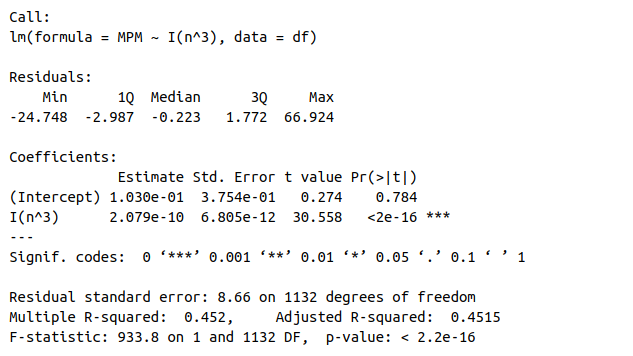
\includegraphics[width=0.55\textwidth]{mpm_n^3_lm.png}
    \captionsetup{justification=centering}
    \caption{Resultado da regressão linear: \\$MPM \sim n^3$}
    \label{fig:mpm-regression}
\end{wrapfigure}

A função Call que vemos nas figuras permite identificar a função e parâmetros que foram utilizados para criar o modelo. No nosso caso as variáveis são o tempo de execução de cada algoritmo em função do número de arestas e do número de vértices.
Os resíduos representam a diferença entre o que o modelo previu e o valor real da variável y. Os coeficientes representam os valores que minimizam a soma do quadrado dos erros.
O Std. Error representa o desvio padrão dividido pela raiz quadrada do tamanho da nossa amostra.
O coeficiente de determinação, consiste numa medida que mostra o quão bem o modelo se ajusta aos dados.

Ao analisar os modelos obtidos, apenas para o caso EK, figura \ref{fig:ek-regression}, conseguimos observar uma boa performance a aproximar os dados com um $R^2 = 0.9352$. Apesar deste bom resultado conseguimos observar que o terceiro coeficiente, $n$, não tem grande impacto no modelo dado o teste estatístico com um valor de $t$ pequeno e estar fora da região crítica ($P = 0.246$).

Nos casos Dinic e MPM, dado os baixos valores de $R^2$, somos levados a questionar os pressupostos de complexidade temporal. Nas próximas sub-secções iremos realizar diferentes transformações para tentar obter um melhor modelo para ambos.





\WFclear
\newpage
\subsection{Transformação Dinic}

\begin{wrapfigure}{R}{0.5\textwidth}
\centering
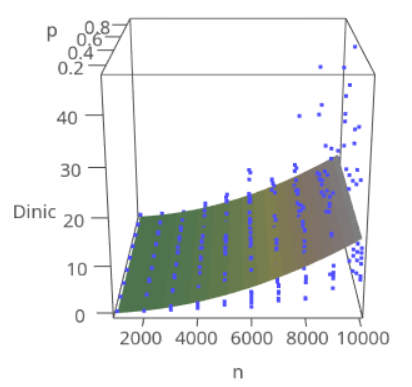
\includegraphics[width=0.45\textwidth]{dinic_n^2_plot_lm.png}
\captionsetup{justification=centering}
\caption{Visualização da regressão linear: \\$Dinic \sim n^2$}
\label{fig:plot3d-dinic}
\end{wrapfigure}

Na tentativa de obter um melhor modelo que se ajuste ao algoritmo Dinic, e ao analisar os vários coeficientes da regressão inicial, ver figura \ref{fig:dinic-regression}, decidimos descartar o 2º coeficiente ($a$) com uma estatística $t = 1.154$.

Como podemos ver pela figura \ref{fig:dinic-regression-2}, conseguimos obter um valor de $R^2$ equiparável, mas que mesmo assim não se revela um bom modelo.
Através do plot "Residuals vs Fitted", figura \ref{fig:dinic-residuals}, que mostra os resíduos no eixo do y e os valores ajustados no eixo do x, é possível ver que existe alguma variabilidade das observações, em contrapartida no início os pontos são semelhantes aos valores ajustados para os pontos da reta de regressão. Por fim, foi possível identificar 3 outliers.

Como se pode ver no plot3D da figura \ref{fig:plot3d-dinic}, quando o nº vértices aumenta o tempo de execução também aumenta. Também é possível observar que, para valores mais altos de número de vértices, existe uma grande variância de tempos de execução.

É importante ainda mencionar que foram feitas várias tentativas de encontrar outros modelos mas nenhum foi superior tanto no valor de $R^2$ como na simplicidade de termos como o aqui apresentado.

\begin{figure}[h]
    \centering
    \begin{minipage}{0.45\textwidth}
        \centering
        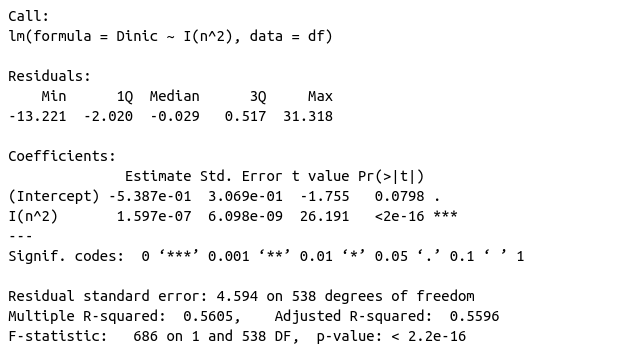
\includegraphics[width=1.2\textwidth]{dinic_n^2_lm.png}
        \captionsetup{justification=centering}
        \caption{Resultado da regressão linear: \\$Dinic \sim n^2$}
        \label{fig:dinic-regression-2}
    \end{minipage}
    \hfill
    \begin{minipage}{0.45\textwidth}
        \centering
        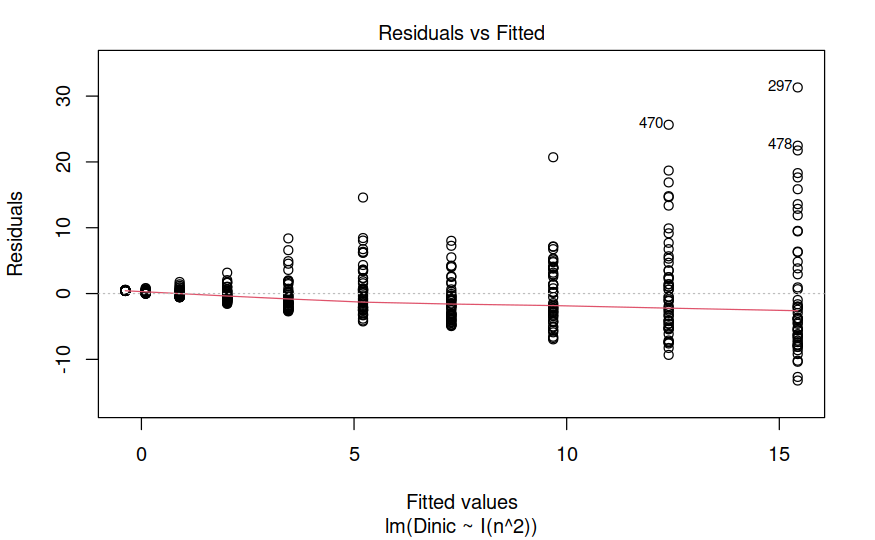
\includegraphics[width=1\textwidth]{dinic_n^2_residuals.png}
        \captionsetup{justification=centering}
        \caption{Visualização dos resíduos: \\$Dinic \sim n^2$}
        \label{fig:dinic-residuals}
    \end{minipage}
\end{figure}





\WFclear
\newpage
\subsection{Transformação EK}

\begin{wrapfigure}{R}{0.5\textwidth}
\centering
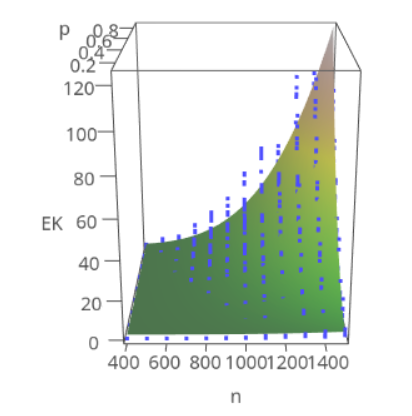
\includegraphics[width=0.45\textwidth]{ek_a^2_plot_lm.png}
\captionsetup{justification=centering}
\caption{Visualização da regressão linear: \\$EK \sim a^2$}
\label{fig:plot3d-ek}
\end{wrapfigure}

Para o algoritmo EK, também procedemos à remoção do termo menos significativo do modelo, $n$ com uma estatística $t=1.161$. Como se pode ver na figura \ref{fig:ek-regression-2}, o desempenho do modelo não é afetada.

Através do plot "Residuals vs Fitted" que está visível na figura \ref{fig:ek-residuals} conseguimos perceber que à medida que avançamos no eixo do x (fitted values) os valores vão oscilando bastante no eixo do y (residuals). Até obtermos o valor 20 no eixo do x, os valores encontram-se todos muito próximos da linha da regressão linear, porém, a partir é possível observar uma maior variância dos dados e até mesmo 3 outliers.

No plot3d, figura \ref{fig:plot3d-ek}, é possível perceber que a valor de número de vértices e probabilidade tem impacto no valor do tempo de execução, na medida em que quanto maior forem ambos os parâmetros, maior vai ser o tempo de execução.

Dado o alto valor de $R^2$ consideramos este modelo um bom aproximador para o comportamento deste algoritmo.

\vspace{0.2\linewidth}
\begin{figure}[h]
    \centering
    \begin{minipage}{0.45\textwidth}
        \centering
        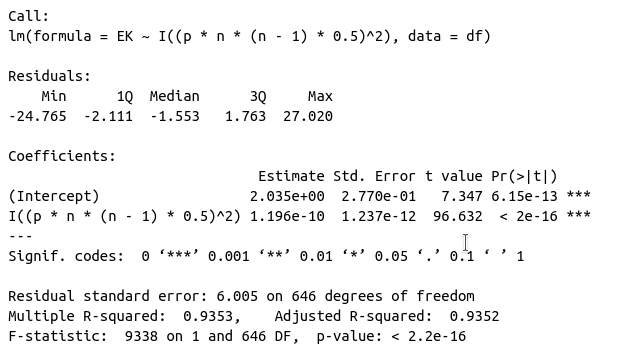
\includegraphics[width=1.2\textwidth]{ek_a^2_lm.png}
        \captionsetup{justification=centering}
        \caption{Resultado da regressão linear: \\$EK \sim a^2$}
        \label{fig:ek-regression-2}
    \end{minipage}
    \hfill
    \begin{minipage}{0.45\textwidth}
        \centering
        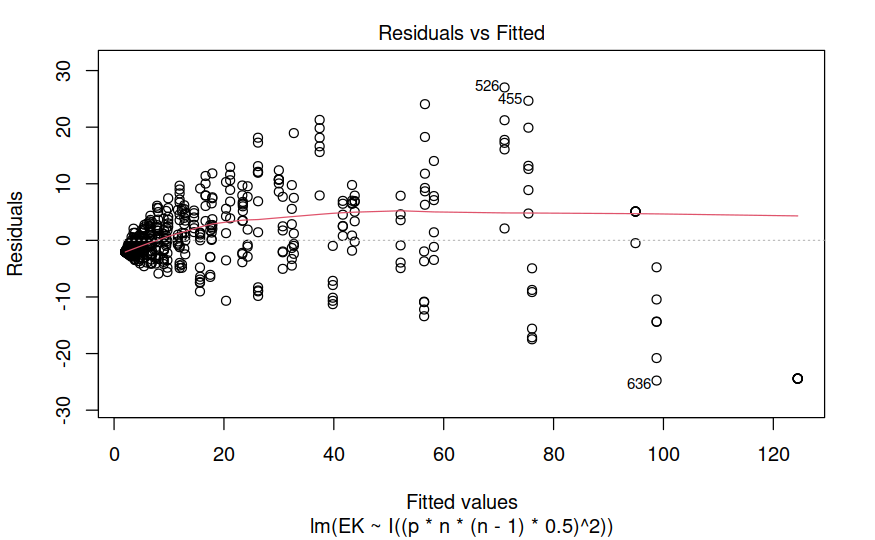
\includegraphics[width=1\textwidth]{ek_a^2_residuals.png}
        \captionsetup{justification=centering}
        \caption{Visualização dos resíduos: \\$EK \sim a^2$}
        \label{fig:ek-residuals}
    \end{minipage}
\end{figure}





\WFclear
\newpage
\subsection{Transformação MPM}

Para o algoritmo MPM, começamos por experiementar um modelo na forma $MPM \sim a + n^3$ onde obtivemos uma melhoria considerável no valor de $R^2 = 0.8961$ mas observamos uma baixa contribuição do coeficiente $n^3$ para o modelo, ver figura \ref{fig:plot3d-mpm} com a visualização do modelo.

Assim procedemos à remoção desse termo e obtivemos um valor de $R^2 = 0.938$ como se pode ver na figura \ref{fig:mpm-regression-2}.
Comparando a visualização do novo modelo, figura \ref{fig:plot3d-mpm-2}, com o anterior (\ref{fig:plot3d-mpm}), é claro que este novo modelo se ajusta mais aos dados experimentais.

No plot "Residuals vs Fitted", figura \ref{fig:mpm-residuals}, conseguimos ver os pontos estão semelhantes aos valores ajustados para os pontos da reta de regressão, embora a variância ainda seja significativa para valores maiores. É possível também identificar 3 outliers.

\begin{figure}[h]
    \centering
    \begin{minipage}{0.45\textwidth}
        \centering
        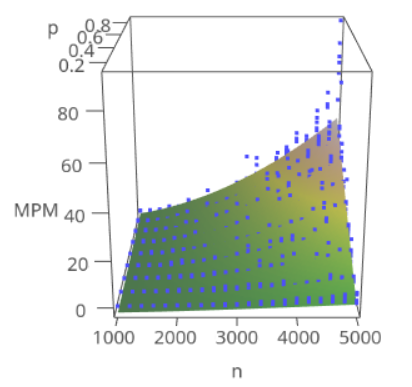
\includegraphics[width=1\textwidth]{mpm_a+n^3_plot_lm.png}
        \captionsetup{justification=centering}
        \caption{Visualização da regressão linear: \\$MPM \sim a + n^3$}
        \label{fig:plot3d-mpm}
    \end{minipage}
    \hfill
    \begin{minipage}{0.45\textwidth}
        \centering
        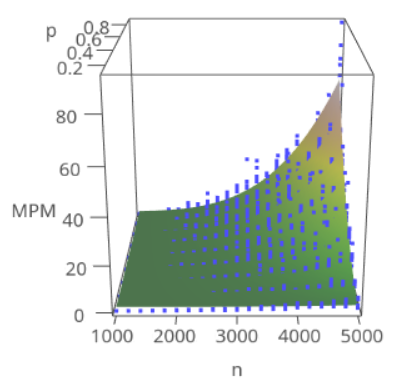
\includegraphics[width=1\textwidth]{mpm_a^2_plot_lm.png}
        \captionsetup{justification=centering}
        \caption{Visualização da regressão linear: \\$MPM \sim a^2$}
        \label{fig:plot3d-mpm-2}
    \end{minipage}
\end{figure}

\begin{figure}[h]
    \centering
    \begin{minipage}{0.45\textwidth}
        \centering
        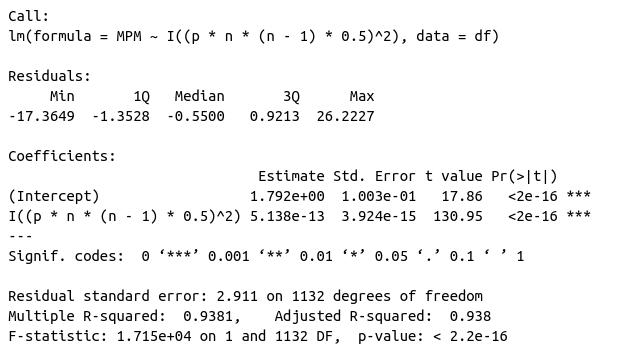
\includegraphics[width=1.1\textwidth]{mpm_a^2_lm.png}
        \captionsetup{justification=centering}
        \caption{Resultado da regressão linear: \\$MPM \sim a^2$}
        \label{fig:mpm-regression-2}
    \end{minipage}
    \hfill
    \begin{minipage}{0.45\textwidth}
        \centering
        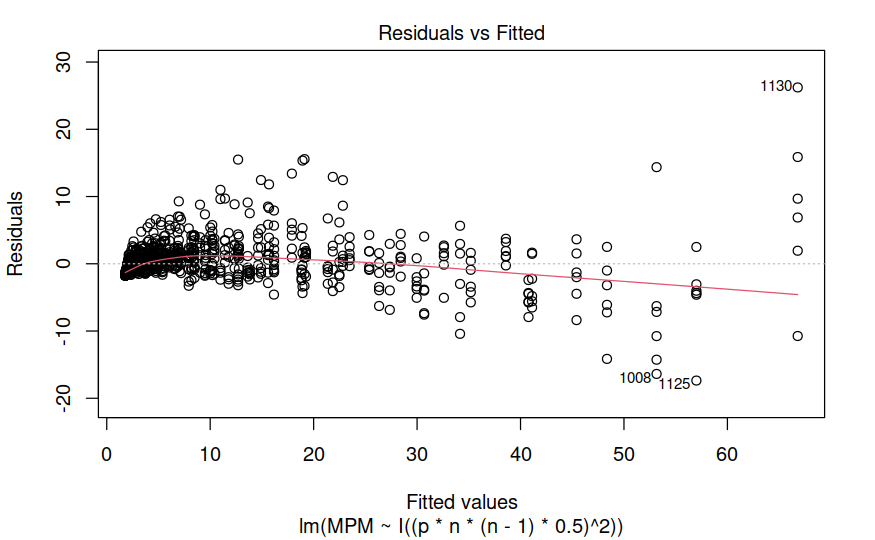
\includegraphics[width=1.1\textwidth]{mpm_a^2_residuals.png}
        \captionsetup{justification=centering}
        \caption{Visualização dos resíduos: \\$MPM \sim a^2$}
        \label{fig:mpm-residuals}
    \end{minipage}
\end{figure}




\WFclear
\newpage
\section{Conclusão}

Com a realização da análise exploratória de dados (EDA) efetuada às diferentes variáveis de estudo, foi possível avaliar a performance dos 3 algoritmos, considerando diferentes parâmetros. 
Numa primeira análise foi importante identificar e perceber as diferentes distribuições dos modelos (linear, quadrática, cúbica)  e o seu comportamento perante diversos fatores, $n$ e $p$.
Esta fase foi particularmente importante para identificar o impacto da variável $p$ nos diversos algoritmos como é descrito a seguir.

Quando aplicamos o modelo de regressão inicial para os 3 algoritmos, ajustados à sua complexidade temporal, foi possível observar algumas diferenças.

Para o algoritmo Dinic, o modelo $Dinic \sim a + n^2$ não se ajusta aos dados pois o seu $R^2$ é relativamente baixo. Foi possível obter um modelo simplificado com o modelo $Dinic \sim n^2$ mantendo o desempenho. É importante notar que o algoritmo Dinic foi o que apresentou maiores variâncias nos tempos de execução e que tal, concluímos, foi a razão para os nossos valores de $R^2$ serem tão pequenos.

Pelo contrário, para o EK o modelo inicial $EK \sim a^2 + n$ apresentou um $R^2$ de 0.9352, o que nos levou a concluir que o algoritmo EK segue efetivamente a complexidade temporal esperada de $O(|V||A|^2)$. Foi ainda possível manter a mesma performance com $EK \sim a^2$.

Em relação ao MPM, que era expectável apresentar uma complexidade temporal cúbica $O(|V|^3)$, foi concluído que o seu tempo de execução afinal depende também do número de arcos do grafo. Esta conclusão foi obtida tanto através da analise EDA como depois na regressão linear. A introdução de $|A|$ como coeficiente (portanto o modelo $MPM \sim a + n^3$) provou novamente o impacto do número de arcos no desempenho algoritmo. De notar que é ainda possível obter um melhor valor de $R^2=0.938$ se elevarmos o coeficiente $|A|^2$, obtendo então o modelo $MPM \sim a^2$.

Por fim, resta concluir que o algoritmo Dinic é sem duvida o mais performante dos três. Tal é possível observar não só nas experiências efetuadas como também nos modelos finais obtidos com as regressões onde o algoritmo Dinic apresenta uma estimativa para o coeficiente quadrático bastante inferior aos restantes ($10^{-7}$ vs $10^{-10}$, no caso EK, e $10^{-13}$, no caso MPM).


\begin{thebibliography}{ht}
\bibitem{texbook}
\emph{R documentation}, \url{https://www.rdocumentation.org/}.

\bibitem{mei-course-materials}
Luís Paquete (2022), Materiais disponibilizados no âmbito da disciplina de MEI

\bibitem{page-wiki-linear-regression}
Various authors, \emph{Wikipedia: Linear regression}, \url{https://en.wikipedia.org/wiki/Linear\_regression}

\bibitem{video-introduction-to-nonlinear-regression}
Edward Roualdes (2020), \emph{A Quick Introduction to Nonlinear Regression}, \url{https://youtu.be/4MFrcfpx7Hg}

\bibitem{video-nonlinear-regression-using-r}
Biplab Bose (2022), \emph{Lec 33: Nonlinear regression using R}, \url{https://youtu.be/v\_VoHgaLkwM}

\bibitem{video-regression-prediction-with-lm}
Equitable Equations (2021), \emph{Regression and Prediction in R Using the lm() Command}, \url{https://youtu.be/sPnS1SlpJvE}

\bibitem{video-linear-regression-summary}
Dataslice (2020), \emph{Linear Regression Summary in R}, \url{https://youtu.be/7WPfuHLCn\_k}

\bibitem{video-linear-regression-plots}
Dataslice (2021), \emph{Linear Regression Plots in R}, \url{https://youtu.be/rfH7pCFvFT0}

\bibitem{page-understanding-diagnostic-plots-regression}
Bommae Kim (2015), \emph{Understanding Diagnostic Plots for Linear Regression Analysis}, \url{https://data.library.virginia.edu/diagnostic-plots/}

\bibitem{page-fiting-a-quadratic-model}
David Lillis, \emph{R Is Not So Hard! A Tutorial, Part 4: Fitting a Quadratic Model}, \url{https://www.theanalysisfactor.com/r-tutorial-4/}

\bibitem{video-intro-r-formulas}
Curtis Miller (2020), \emph{Intro R: Formulas}, \url{https://youtu.be/4Zy5x\_cFz1g}

\end{thebibliography}

\appendix

\section{Alterações realizadas}

\begin{itemize}
    \item Correção da estimativa para $|A|$, o número de arcos do grafo, como $|A|=p\frac{n(n-1)}{2}$ em vez de $|A|=np$;
    \item Foram realizados testes adicionais para os algoritmos Dinic e MPM para valores de $p \in [0.1, 0.9]$, anteriormente apenas tinhamos realizado a análise para o intervalo $p \in [0.3, 0.7]$;
    \item Foram atualizados os diferentes boxplots que compõem a EDA dados os novos intervalos para a variável $p$;
    \item Foram calculadas novas regressões para os vários algoritmos: concluímos que o algoritmo Dinic seguia um modelo $O(|V|^2)$ e não o esperado $O(|A||V|^2)$; que o algoritmo MPM segue uma complexidade de $O(|A|^2)$ e não $O(|V|^3)$; e que o algoritmo EK segue a complexidade esperada de $O(|V||A|^2)$;
    \item No seguimento das novas regressões foram atualizados os diferentes gráficos que compõem a EDA (boxplots, scaterplots e residuals vs fitted.
\end{itemize}

\end{document}
